\lhead{\textit{NOTATION SYMBOLIQUE}}
La notation \textit{symbolique} de la Musique a pour but d'être lue, comprise et interprétée par les humains.  
Après s'être intéressé aux outils actuels de création musicale, cette section décrit les outils informatiques existants pour une notation traditionnelle et symbolique de la musique. 
En prenant en compte les challenges soulevés par la musique contemporaine (voir section\ref{subsec:tendancesNotationnellesXX}), les outils présentés dans cette section seront évaluées en fonction des critères suivants :
Est-ce que le logiciel permet la création de nouveaux symboles musicaux? Permet-il d'associer une sémantique aux nouveaux symboles créés?
A savoir, ces outils proposent-ils des moyens d'adaptation et d'augmentation de la notation standard?

\subsection{Outils de notation à base de compilateurs}
\label{subsec:notationABaseCompilateurs}
Un premier type de logiciels, proposant une notation symbolique de la Musique, permet de décrire textuellement une partition, puis de compiler le texte pour générer le résultat graphique.
De nombreux paramètres de mise en page de la partition sont gérés automatiquement à la compilation (espacement des notes, gestion des retours à la ligne…).

\paragraph{MusiXTeX} Le langage MusiXTeX, basé sur le processeur de texte \TeX, est un des outils permettant de générer une portée graphique à partir de texte. MusiXTeX a besoin de trois passes de compilation (1 passe \TeX, 1 passe \textit{musicflx}, et 1 passe \TeX) pour pouvoir calculer un espacement horizontal adéquat entre les notes et ensuite générer le document PDF \cite{musixtex2016}.

MusiXTeX fournit les symboles de la notation standard, ainsi que des symboles musicaux moins répandus, accessibles dans ses nombreuses extensions (par exemple, l'extension \textit{musixgre} permet l'utilisation de la notation carrée, voir la section \ref{sec:unPeuDHistoire}).
Pour représenter les notes, MusiXTeX utilise le système anglo-saxon (maintenant système international), dans lequel les sept premières lettres de l'alphabet $a, b, c, d, e, f, g$ correspondent respectivement aux notes la, si, do, ré, mi, fa, sol. Pareillement, les valeurs rythmiques de notes sont introduites par les balises \lstinline{\wh} (ronde, \textit{whole note}), \lstinline{\h} (blanche, \textit{half note} en anglais), \lstinline{\q} (noire, \textit{quarter note} en anglais)… 

MusiXTeX ne permet pas la création de nouveaux symboles pour la portée, et l'intégration de symboles écrits avec d'autre package \LaTeX, comme \textit{tikz}, est complexe voir impossible.
Aussi, le rendu final de la compilation est un fichier PDF, donc un format purement graphique. La partition produite n'est pas interprétable par ordinateur.

\paragraph{Lilypond} Lilypond est un autre générateur de portée, logiciel libre rattaché au projet \textit{GNU} \cite{lilypond2018}. Son système de notation est semblable à celui de MusiXTeX (il existe d'ailleurs un package Lilypond pour \LaTeX), avec plus de légèreté syntaxique, et une communauté d'utilisateurs et de développeurs bien plus active.

Lilypond fournit son propre compilateur (le binaire \textit{lilypond}) pour générer un fichier pdf en sortie. Un fichier MIDI correspondant à la partition peut également être généré; la partition est donc interprétable par ordinateur.
L'utilisateur peut modifier à son aise les propriétés graphiques des éléments de la partition, et même créer de nouveaux symboles à l'aide de la balise \lstinline|\markup nomDuSymbole args|. Grâce à cette possibilité d'augmentation de la portée par de nouveaux symboles, il existe de nombreux exemples de pièces contemporaines notées avec Lilypond. Pour l'exemple, une pièce de Mike Solomon est visible en annexe \ref{sec:luckyWokSolomon}.

De plus, le compilateur Lilypond inclus le moteur \textit{Guile}, implémentation du langage \textit{Scheme}, qui permet l'intégration de scripts \textit{Scheme} à la syntaxe Lilypond. De fait, les capacités algorithmiques d'un langage de programmation générique sont mises au service de l'écriture de partition.

Cependant, et c'est la critique majeure qui peut être adressée aux systèmes à compilateur, la définition de nouveaux symboles graphiques reste complexe, et nécessite d'être rompu à la pratique des langages de programmation.
De même, lorsqu'un nouveau symbole est créé, Lilypond ne permet pas de lui associer une sémantique, qui lui permettrait, par exemple, d'être transcrit au format MIDI et interprété par l'ordinateur.

\paragraph{GUIDO} GUIDO, spécifié à l'origine par Holger H. Hoos et Keith Hamel, est un format pour la notation de la musique \cite{hoos1998}. Lors de sa création, GUIDO n'était accompagné d'aucun compilateur permettant de générer un rendu graphique ou sonore à partir du texte. Par la suite, le GUIDO Engine a été développé par le SALIERI Group puis le GRAME (centre national de création musicale basé à Lyon), pour permettre la visualisation graphique de la portée à partir du format spécifié. 

Même si ce format ne permet aucune intégration de nouveaux symboles, ni de convertir le texte en un format sonore, la concision de sa syntaxe et l'existence de SDKs pour le GuidoEngine en font un outil facilement intégrable dans un logiciel de notation musicale. Par exemple, l'environnement pour partition augmentée Inscore (voir section ), aussi développé par le GRAME, utilise le format GUIDO pour la partie notation standard de la Musique.    

\subsection{Outils de notation wysiwyg}
\label{subsec:outilsWysiwyg}

De nombreux outils de notation musicale wysiwyg (pour \textit{what you see is what you get}) existent dans le domaine libre et commercial. Parmi les plus populaires, \textit{Finale} (MakeMusic) et \textit{Sibelius} (Avid) sont des logiciels propriétaires payants, et \textit{Musescore} et \textit{NoteAbility Pro} font partie du monde libre.

Leur interface graphique présente les mêmes caractéristiques : la portée fait office d'élément central, accompagnée d'une palette des symboles inscriptibles et d'un lecteur permettant de jouer la partition.
Les logiciels wysiwyg de notation incluent systématiquement un moteur d'interprétation MIDI pour le rendu audio de la pièce musicale.
La figure \ref{fig:sibeliusScreenshot} donne une vue du logiciel Sibelius présentant les éléments cités ci-dessus.

\begin{figure}[H]
	\centering
	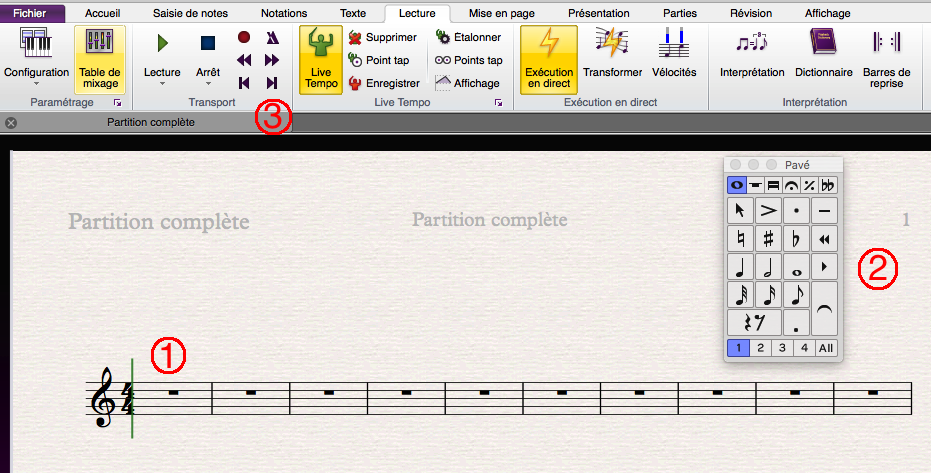
\includegraphics[keepaspectratio=true, width=0.7\textwidth]{OutilsInformatiques/i/sibeliusScreenshot.png}
	\caption{Capture d'écran du logiciel Sibelius}
	\label{fig:sibeliusScreenshot}
	\small \it
	En 1, la portée. En 2, la palette (appelé "pavé" dans Sibelius) des symboles de la notation standard.
	En 3, la barre de transport permettant la lecture et le jeu de la partition. 			
\end{figure}

L'interface graphique de tels logiciels facilite l'écriture de partitions par tous types d'utilisateurs-musiciens, là où les outils de notation à compilateur nécessitaient une connaissance de la programmation informatique.

Cependant, les logiciels actuels ne permettent que très difficilement de sortir des sentiers battus de la notation standard pour créer de nouveaux symboles et leur associer une sémantique. Les trois systèmes les plus répandus que sont \textit{Sibelius}, \textit{Finale} et \textit{Musescore} proposent la fonctionnalité d'insertion d'images pour ajouter de nouvelles entités musicales à une partition. En revanche, la palette ne peut pas être étendue par de nouveaux symboles, et la modification du graphisme des figures existantes ne fait pas partie du comportement naturel de ces programmes. Un bémol est à ajouter à cette déclaration en prenant en compte l'intégration par \textit{Finale} d'un véritable éditeur graphique dans son interface, permettant aux utilisateurs de créer leurs propres symboles et de les sauvegarder dans leur palette (le compositeur Alireza Farhang utilise cette fonctionnalité pour créer des symboles inédits, voir annexe \ref{sec:exempleAlirezaFarhang}).

\paragraph{NoteAbility} Le logiciel \textit{NoteAbility} fait figure d'exception en ce qu'il offre à l'utilisateur une grande liberté dans la modification du graphisme de la portée et des symboles musicaux \cite{noteAbility2018}.
Il intègre même des outils d'édition graphique qui confère la possibilité de dessiner à même la portée.
Également, une sémantique particulière peut être associée à des symboles en leur adjoignant des messages, qui seront envoyés sur un port UDP particulier lors de la lecture. Ces messages peuvent être reçus par n'importe quel logiciel écoutant le port en question, et transcris en interprétation sonore.

Toutefois, \textit{NoteAbility} ne permet pas de sauvegarder les nouveaux symboles créés dans la palette des \textit{Music Images} (terme utilisé pour qualifier les symboles musicaux). Cette fonctionnalité est annoncée pour les versions à venir.      